%% Преамбула TeX-файла

% 1. Стиль и язык
\documentclass[utf8x]{G7-32} % Стиль (по умолчанию будет 14pt)
\usepackage[T2A]{fontenc}
\usepackage[russian]{babel}
% Остальные стандартные настройки убраны в preamble.inc.tex.
\sloppy

% Настройки стиля ГОСТ 7-32
% Для начала определяем, хотим мы или нет, чтобы рисунки и таблицы нумеровались в пределах раздела, или нам нужна сквозная нумерация.
\EqInChapter % формулы будут нумероваться в пределах раздела
\TableInChapter % таблицы будут нумероваться в пределах раздела
\PicInChapter % рисунки будут нумероваться в пределах раздела

% Добавляем гипертекстовое оглавление в PDF
\usepackage[
bookmarks=true, colorlinks=true, unicode=true,
urlcolor=black,linkcolor=black, anchorcolor=black,
citecolor=black, menucolor=black, filecolor=black,
]{hyperref}

% Изменение начертания шрифта --- после чего выглядит таймсоподобно.
% apt-get install scalable-cyrfonts-tex

\IfFileExists{cyrtimes.sty}
    {
        \usepackage{cyrtimespatched}
    }
    {
        % А если Times нету, то будет CM...
    }

\usepackage{graphicx}   % Пакет для включения рисунков

% С такими оно полями оно работает по-умолчанию:
% \RequirePackage[left=20mm,right=10mm,top=20mm,bottom=20mm,headsep=0pt]{geometry}
% Если вас тошнит от поля в 10мм --- увеличивайте до 20-ти, ну и про переплёт не забывайте:
\geometry{right=20mm}
\geometry{left=30mm}


% Пакет Tikz
\usepackage{tikz}
\usetikzlibrary{arrows,positioning,shadows}

% Произвольная нумерация списков.
\usepackage{enumerate}

% ячейки в несколько строчек
\usepackage{multirow}

% itemize внутри tabular
\usepackage{paralist,array}


% Настройки листингов.
% 8 Листинги

\usepackage{listings}

% Значения по умолчанию
\lstset{
  basicstyle= \footnotesize,
  breakatwhitespace=true,% разрыв строк только на whitespacce
  breaklines=true,       % переносить длинные строки
%   captionpos=b,          % подписи снизу -- вроде не надо
  inputencoding=koi8-r,
  numbers=left,          % нумерация слева
  numberstyle=\footnotesize,
  showspaces=false,      % показывать пробелы подчеркиваниями -- идиотизм 70-х годов
  showstringspaces=false,
  showtabs=false,        % и табы тоже
  stepnumber=1,
  tabsize=4,              % кому нужны табы по 8 символов?
  frame=single
}

% Стиль для псевдокода: строчки обычно короткие, поэтому размер шрифта побольше
\lstdefinestyle{pseudocode}{
  basicstyle=\small,
  keywordstyle=\color{black}\bfseries\underbar,
  language=Pseudocode,
  numberstyle=\footnotesize,
  commentstyle=\footnotesize\it
}

% Стиль для обычного кода: маленький шрифт
\lstdefinestyle{realcode}{
  basicstyle=\scriptsize,
  numberstyle=\footnotesize
}

% Стиль для коротких кусков обычного кода: средний шрифт
\lstdefinestyle{simplecode}{
  basicstyle=\footnotesize,
  numberstyle=\footnotesize
}

% Стиль для BNF
\lstdefinestyle{grammar}{
  basicstyle=\footnotesize,
  numberstyle=\footnotesize,
  stringstyle=\bfseries\ttfamily,
  language=BNF
}

% Определим свой язык для написания псевдокодов на основе Python
\lstdefinelanguage[]{Pseudocode}[]{Python}{
  morekeywords={each,empty,wait,do},% ключевые слова добавлять сюда
  morecomment=[s]{\{}{\}},% комменты {а-ля Pascal} смотрятся нагляднее
  literate=% а сюда добавлять операторы, которые хотите отображать как мат. символы
    {->}{\ensuremath{$\rightarrow$}~}2%
    {<-}{\ensuremath{$\leftarrow$}~}2%
    {:=}{\ensuremath{$\leftarrow$}~}2%
    {<--}{\ensuremath{$\Longleftarrow$}~}2%
}[keywords,comments]

% Свой язык для задания грамматик в BNF
\lstdefinelanguage[]{BNF}[]{}{
  morekeywords={},
  morecomment=[s]{@}{@},
  morestring=[b]",%
  literate=%
    {->}{\ensuremath{$\rightarrow$}~}2%
    {*}{\ensuremath{$^*$}~}2%
    {+}{\ensuremath{$^+$}~}2%
    {|}{\ensuremath{$|$}~}2%
}[keywords,comments,strings]

% Подписи к листингам на русском языке.
\renewcommand\lstlistingname{\cyr\CYRL\cyri\cyrs\cyrt\cyri\cyrn\cyrg}
\renewcommand\lstlistlistingname{\cyr\CYRL\cyri\cyrs\cyrt\cyri\cyrn\cyrg\cyri}


% Полезные макросы листингов.
% Любимые команды
\newcommand{\Code}[1]{\textbf{#1}}

\newcommand{\myImage}[3]{
\begin{figure}[!ht]
    \centering
    \includegraphics[width=\textwidth]{figures/#2}
    \caption{#1}
    \label{#3}
\end{figure}
}


% Пакет для листингов кода
\usepackage{verbatim}
\usepackage{float}
\floatstyle{ruled}
\newfloat{program}{th}{lop}
\floatname{program}{Листинг}


\newtheorem{theorem}{Теорема}
\newtheorem{definition}{Определение}

\begin{document}

\pagestyle{empty}
\begin{center}
  Министерство образования и науки Российской Федерации\\
  ФГАОУ ВПО  «УрФУ имени первого Президента России Б. Н. Ельцина»\\
  Институт радиоэлектроники и информационных технологий - РтФ\\
  Департамент информационных технологий и автоматики
  \par
  \vspace{4.5cm}
  \Large{
    Исследование предельных циклов нелинейной системы

    \par
    \vspace{0.5cm}

    ОТЧЕТ\\
    по лабораторной работе
  }

  \vspace{4cm}
  {
    Преподаватель: \hfill Пименов Владимир Германович
  }
  \par
  {
    Студент: \hfill Сухоплюев Илья Владимирович
  }
  \par
  {
    Группа: \hfill РИ-440001
  }

  \par
  \vspace{3.5cm}
  Екатеринбург\\
  2017
\end{center}


\frontmatter % выключает нумерацию ВСЕГО; здесь начинаются ненумерованные главы: реферат, введение, глоссарий, сокращения и прочее.

% Команды \breakingbeforechapters и \nonbreakingbeforechapters
% управляют разрывом страницы перед главами.
% По-умолчанию страница разрывается.

% \nobreakingbeforechapters
% \breakingbeforechapters

\begin{abstract}

Работа описывает исследование параметризованной нелинейной системы
на наличие предельных циклов. В ходе исследования системы,
рассматриваются следующие вопросы: нахождение параметра системы, при котором 
наблюдается предельный цикл; поиск параметра, где наблюдается бифуркация поведения системы;
исследование свойств обнаруженного предельного цикла и определение характера его
устойчивости. Данные задачи изучаются путем проведения численных экспериментов
с помощью интерпретатора Python 3.5 и математических библиотек (numpy\cite{numpy},
matplotlib\cite{matplotlib}).

\end{abstract}

%%% Local Variables: 
%%% mode: latex
%%% TeX-master: "rpz"
%%% End: 


\pagestyle{plain}

\tableofcontents

\mainmatter % это включает нумерацию глав и секций в документе ниже

\chapter{Поиск предельного цикла}

Рассмотрим исследуемую систему (уравнение \eqref{lab:eq:1},
$\nu$ - параметр системы). Она описывается
уравнением от одной фазовой переменной $x$. Уравнение дифференциальное, второго
порядка и, в силу слагаемого $3\dot{x}^3$, нелинейное. Решение такого уравнения
аналитическими методами является довольно сложной задачей, поэтому нашим
методом исследования будет построение численных экспериментов, описывающих
данную систему при определенном параметре $\nu$.

\begin{equation}\label{lab:eq:1}
  \ddot{x} + 3 \dot{x}^3 - \nu\dot{x} + x = 0
\end{equation}

Однако, в таком виде уравнение \eqref{lab:eq:1} не является удобным для
моделирования. Поэтому приведем его к канонической форме от двух переменных, с
помощью замены \eqref{lab:eq:2}, получив уравнение от двух фазовых переменных
$y_1$ и $y_2$ (Система уравнений \eqref{lab:eq:3}). В дальнейшем, мы будем
пользоваться описанием нашей системы именно в таком виде.

\begin{equation}\label{lab:eq:2}
  \begin{cases}
    &y_1 = x \\
    &y_2 = \dot{x}
  \end{cases}
\end{equation}

\begin{equation}\label{lab:eq:3}
  \begin{cases}
    &\dot{y_1} = y_2 \\
    &\dot{y_2} = -3y_2^3\ + \nu y_2 - y_1
  \end{cases}
\end{equation}

Преобразовав систему к удобному для нас виду, перейдем к первой части работы --
нахождения такого параметра $\nu$, при котором наблюдается предельный цикл.

Для начала, дадим определение искомому объекту.

\begin{definition}\label{lab:def:cycle}
  Предельным циклом будем называть замкнутую изолированную траекторию
  в фазовом пространстве, подразумевая замкнутость в смысле периодичности
  поведения системы.
\end{definition}

Таким образом, нам нужно построить фазовый портрет нашей системы, на котором
нужно будет обнаружить искомую замкнутую линию. Для этого, зная зависимость
значения производных от их координат, можно с помощью функции
\textit{streamplot}\cite{streamplot} построить фазовый портрет (Программа
\ref{lab1:prog:1}, в качестве параметра для начала возьмем $\nu = 1$).

\begin{program}
  \caption{Построение фазового портрета}
  \label{lab1:prog:1}
  \begin{verbatim}
# Подключение используемых библиотек
# В дальнейшем является постоянным и опускается в листингах
# Полный исходный код программы можно найти в приложении
import matplotlib.pyplot as plt
import numpy as np

# Параметр системы
nu = 1

# создание сетки 100х100 точек в области [-3;3]x[-3;3]
Y, X = np.mgrid[-3:3:100j, -3:3:100j]

# вычисление фазовых векторов на сетке
Y1 = Y
Y2 = -3 * Y ** 3 + nu * Y - X

# построение фазового портрета
fig0, ax0 = plt.subplots()
plt.streamplot(X, Y, Y1, Y2)

# показать построенные графики (опускается в дальнейшем)
plt.show()
  \end{verbatim}
\end{program}
\clearpage


\begin{figure}[thp]
  \centering
  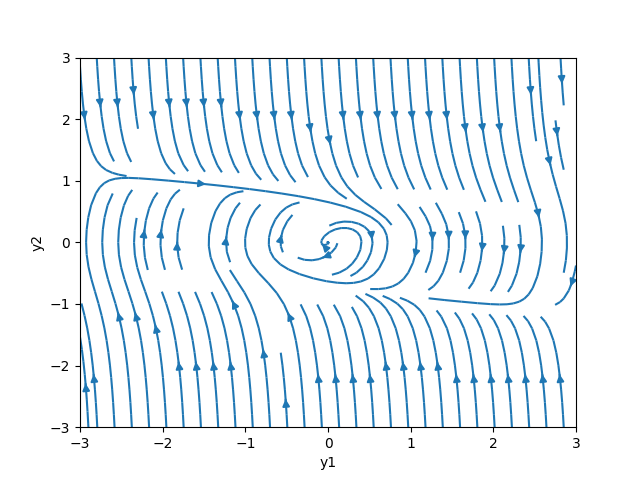
\includegraphics[width=\textwidth]{figures/1_streamplot}
  \caption{Поиск предельного цикла построением фазового портрета}
  \label{lab1:streamplot}
\end{figure}

На графике \ref{lab1:streamplot} изображен результат работы нашей программы.
В данном случае значение параметра оказалось оптимальным: можно видеть, как
изоклины сходятся к наклоненному прямоугольнику в центре графика.

Теперь, чтобы убедится наверняка, что траектории сходятся вокруг этого цикла
и там нет разрывов, построим две линии методом Эйлера снаружи и внутри наблюдаемого
цикла (Программа \ref{lab1:prog:2}).

\begin{program}
  \caption{Использование метода Эйлера для проверки предельного цикла}
  \label{lab1:prog:2}
  \begin{verbatim}
# функция построение кривой методом Эйлера
def line(y1_0, y2_0):
    y1 = [y1_0]
    y2 = [y2_0]
    h = 0.01 # длина шага
    for i in range(2000): # 2000 - количество итераций
        y1.append(y1[i] + h*(y2[i]))
        y2.append(y2[i] + h*(-3*y2[i] ** 3 + nu*y2[i] - y1[i]))
    # отображение кривой на графике
    ax0.plot(y1, y2)

# построение двух кривых, начинающихся внутри и
# вне предполагаемого предельного цикла
line(0.1, 0.1)
line(2, 2)
  \end{verbatim}
\end{program}

\clearpage

\begin{figure}[thp]
  \centering
  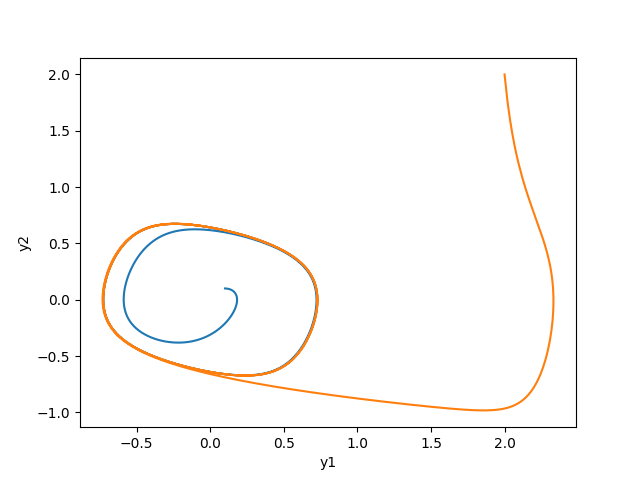
\includegraphics[width=\textwidth]{figures/1_cycle}
  \caption{Обнаружение аттрактора методом Эйлера}
  \label{lab1:cycle}
\end{figure}

На рисунке \ref{lab1:cycle} мы можем видеть две линии, начинающиеся из точек
$(0.1, 0.1)$ и $(2, 2)$. Эти линии сходятся сближаются к искомому предельному
циклу системы.

\chapter{Поиск точек бифуркаций}

Найдя предельный цикл в системе \eqref{lab:eq:3}, мы можем перейти к следующему
этапу нашего исследования -- определения всех значений параметра, при которых
наблюдается данный цикл.

В силу того, что наша система рассматривается дифференциальным уравнением,
поведение системы будет меняться плавно на промежутках, разделенных так
называемыми точками \textit{бифуркации}(точки, в которых происходит изменение
поведения системы).

\begin{definition}
    Точка бифуркации - значение параметра системы, при котором наблюдается
    качественное изменение поведения системы.
\end{definition}

Чтобы нам было удобно наблюдать изменение системы от параметра без перезапуска
программы, мы обернем построения в функцию и добавим в нашу программу слайдер --
бегунок, которым можно будет менять значение параметра $\nu$.

\begin{figure}
    \centering
    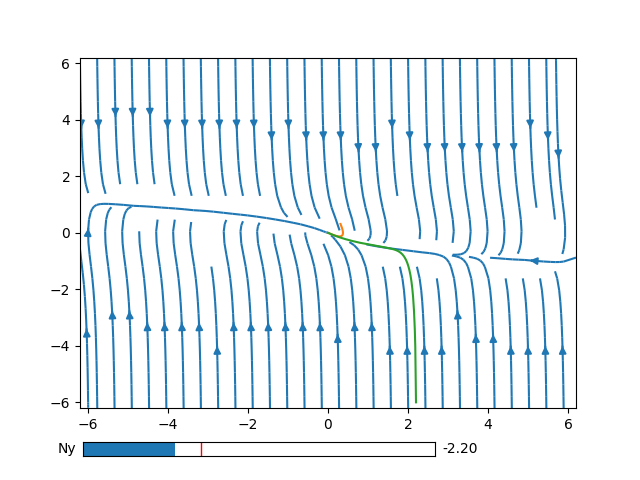
\includegraphics[width=0.8\textwidth]{figures/2_point_-2_2}
    \caption{Стационарная точка системы при $\nu = -2.2$}
    \label{lab2:point_-2}
\end{figure}

Начиная с отрицательных значений (от -10) мы наблюдаем сильное стремление
к центру координат -- стационарной точки системы (График \ref{lab2:point_-2}).

\begin{figure}[!ht]
    \centering
    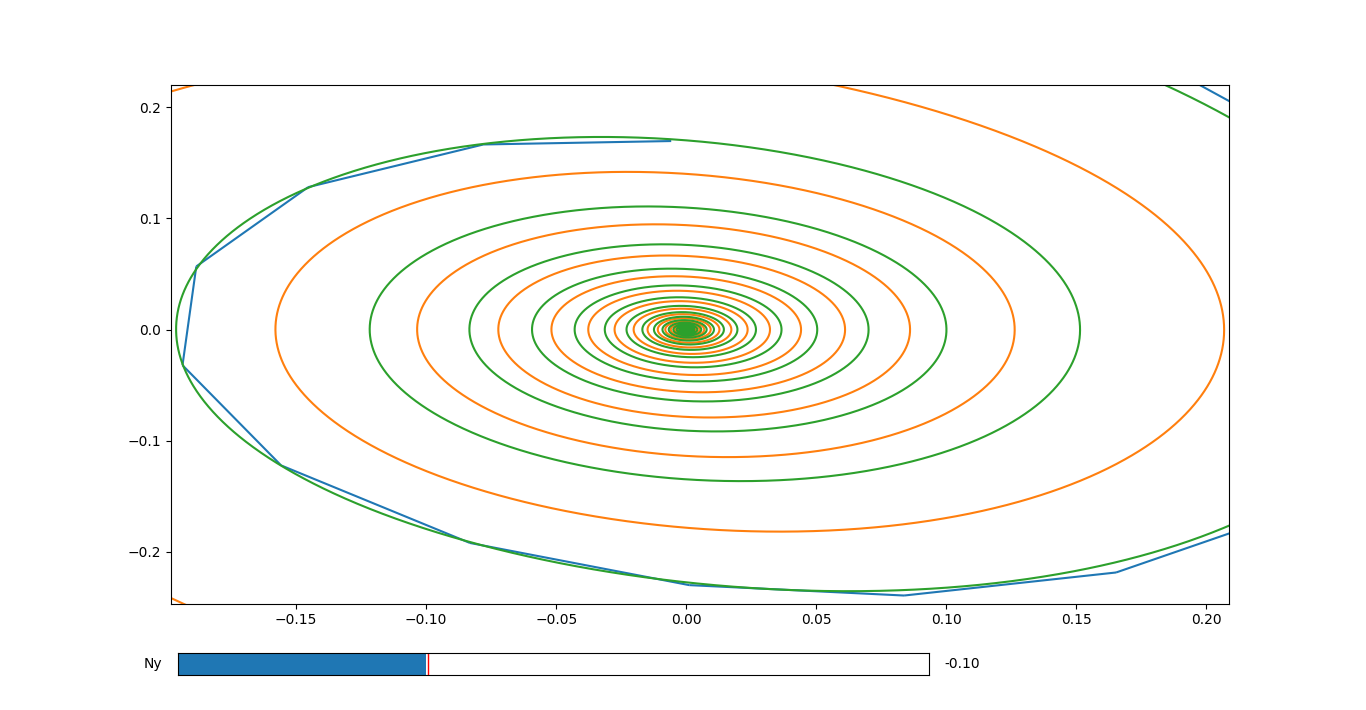
\includegraphics[width=0.8\textwidth]{figures/2_point_-0_1}
    \caption{Стационарная точка системы при $\nu = -0.1$}
    \label{lab2:point_0}
\end{figure}

При приближении параметра к нулю, поведение системы искривляется в овальную
форму, но линии медленно сходятся к нулю (График \ref{lab2:point_0}).

\begin{figure}[!ht]
    \centering
    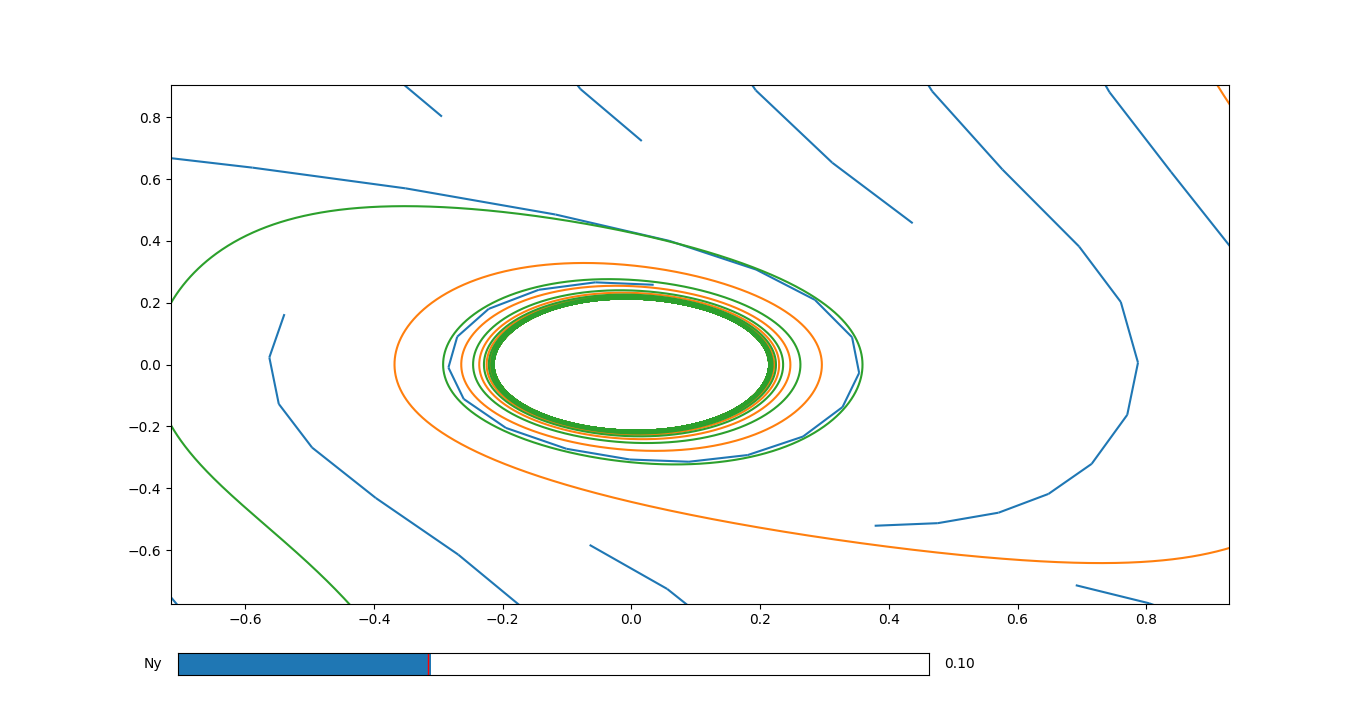
\includegraphics[width=0.8\textwidth]{figures/2_cycle_0_1}
    \caption{Появление цикла при $\nu = 0.1$}
    \label{lab2:cycle_0_1}
\end{figure}

Как только мы переступаем нулевое значение параметра, наши траектории
останавливаются значительно раньше -- мы начинаем наблюдать знакомый нам
предельный цикл, но в меньших размерах (График \ref{lab2:cycle_0_1}).

\begin{figure}[!ht]
    \centering
    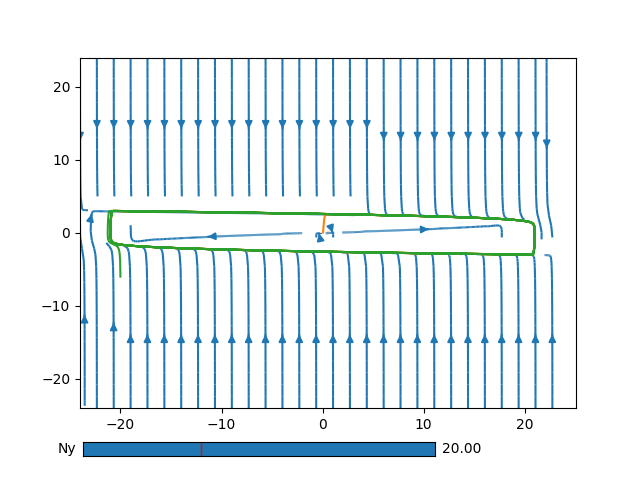
\includegraphics[width=0.8\textwidth]{figures/2_cycle_20}
    \caption{Расширение предельного цикла при увеличении параметра ($\nu = 20$)}
    \label{lab2:cycle_20}
\end{figure}

Увеличивая $\nu$ дальше, остается наблюдать за ростом цикла (График
\ref{lab2:cycle_20}).

Из полученных наблюдений можно выдвинуть гипотезу: на отрицательной полуоси
исследуемая система сходится в стационарную точку; в положительной же оси
наблюдается предельный цикл, который увеличивается в зависимости от параметра
системы.

Стоит отметить, что наличие или отсутствие предельного цикла на границе
($\nu = 0$) мы выявить не можем, так как при приближении к параметра к нулю,
чтобы быть уверенным в наличии стационарной точки или цикла, приходится
увеличивать точность вычислений. В конце концов, когда точность увеличить
не удается, нам остается только предполагать: толи линии сошлись к циклу, толи
они не достигли нуля из-за недостаточного кол-ва шагов в методе Эйлера.

С учетом этого замечания, можно выдвинуть еще одну гипотезу: так как изменение
поведения в системе происходит настолько плавно, что нам не удается уловить
момент, когда мы наблюдаем стационарную точку, а когда предельный цикл.
То есть мы можем говорить, что наблюдается \textit{мягкая бифуркация системы}.

\chapter{Исследование свойств предельного цикла}

Следующим шагом в исследовании системы станет изучение свойств нашего
предельного цикла при конкретном значении параметра (возьмем $\nu = 1$):
нахождение его периода (от независимой переменной) и его форму. Данные свойства
потребуются в следующих частях (\ref{lab4} и \ref{lab5}) для проверки
характера его устойчивости.

Ставя численные эксперименты, значения могут получатся точные, но все же с
погрешностью. Поэтому далее мы будем находить значение с точностью до 3-х знаков
после запятой (т. е. наше значение должно расходится не более чем на
$\epsilon = 0.5 * 10 ^{-4}$).

В программе \ref{lab3:prog:1} строится цикл методом точечных отображений Пуанкаре:
выбирается точка на оси $0_{y1}$, от которой мы начинаем двигаться по траектории
до тех пор, пока снова не пересечет ось. При приближении к нашему предельному
циклу, точки будут сближаться все больше и больше. Таким образом будем считать
траекторию предельным циклом, когда начальная и конечная точка сблизятся по
обоим координатам ближе чем на $\epsilon$. Периодом нашего цикла будет
количество затраченных шагов ($i + 1$) помноженных на длину шага $h$.
Как видно из работы программы, цикл имеет период $\omega = 6.663$.

Далее можно попытаться найти аналитическую форму данного цикла, но судя по
графику \ref{lab1:cycle} форма цикла не похожа на знакомые квадратичные функции и
подбор аналитического вида кривой может оказаться трудной задачей. При этом мы
не сможем достигнуть такой же точности, как наше поточечное решение, полученное
методом Эйлера. Поэтому в следующих работах будем работать с массивами $y1$ и
$y2$, описывающие наш цикл.

\begin{program}
    \caption{Поиск параметров системы}
    \label{lab3:prog:1}
    \begin{verbatim}
eps = 0.5 * 10 ** -4
y1_0, y2_0 = 0.72424, 0 # начальная точка

y1 = [y1_0]
y2 = [y2_0]
h = 0.0001
for i in range(100000):
    # итерация метода Эйлера
    y1.append(y1[i] + h*(y2[i]))
    y2.append(y2[i] + h*(-3*y2[i] ** 3 + ny * y2[i] - y1[i]))
    # проверка прихода в туже точку с погрешностью
    if  np.abs(y1_0 - y1[i+1]) < eps and
        np.abs(y2_0 - y2[i+1]) < eps:
        # вывод результатов
        print("h={h}, i={i}, h*i={period}".format(
              h=h, i=i+1, period=h*(i+1)))
        return;
# Вывод программы
# h=0.0001, i=66633, h*i=6.6633000000000004
    \end{verbatim}
\end{program}



\chapter{Определение устойчивости через мультипликаторы системы}\label{lab4}

В этом разделе будет проведено исследование нашего предельного цикла
на асимптотическую орбитальную устойчивость. Проверку будем проводить с помощью
аналога теоремы Андронова-Витта, вычислив мультипликаторы системы первого
приближения вдоль исследуемого предельного цикла.

Дадим необходимые для этого определения\cite{bookdiff}, относительно системы
дифференциальных уравнений \eqref{lab4:eq:du}.

\begin{equation}\label{lab4:eq:du}
    \dot{x} = f(x), \quad x \in R^n \quad f \in C[R^n]
\end{equation}

\begin{definition}
    Пусть $x = \eta(t)$ - решение системы \eqref{lab4:eq:du},
    определенное при $t > 0$. \textbf{Положительной полутраекторией}
    решения назовем множество в фазовом пространстве:
    \begin{equation*}
        L^+[\eta(\cdot)] = \{x\in R^n, \quad x = \eta(t), \quad t \geq 0\}.
    \end{equation*}
\end{definition}

\begin{definition}
    Решение $\eta(t)$ системы \eqref{lab4:eq:du} называется
    \textbf{орбитально устойчивым} при $t \rightarrow \infty$,
    если для любого $\epsilon > 0$ найдется $\delta > 0$
    такое, что для всех других решений $x(t)$
    системы \eqref{lab4:eq:du} c условием \\
    $||x(0) - \eta(0)|| < \delta$ выполняется
    $\rho(x(t), L^+[\eta(\cdot)]) < \epsilon$ для всех $t \geq 0$.
    Здесь $\rho(x,L)$ означает расстояние от точки $x$ до множества
    $L$ в пространстве $R^n$.
\end{definition}

\begin{definition}
    Орбитально устойчивое решение $\eta(t)$ называется
    \textbf{асимптотически орбитально устойчивым},
    если существует $\Delta > 0$ такое, что для всех решений
    $x(t)$, удовлетворяющих соотношению $||x(0) - \eta(0)|| < \Delta$,
    выполняется предельное соотношение $\rho(x(t), L^+[\eta(\cdot)]) \rightarrow 0$
    при $t \rightarrow \infty$.
\end{definition}

Из поставленных определений видна мотивация исследования решения на наличие
асимптотической орбитальной устойчивости: подтвердив его, мы, увеличивая
точность вычислений, будем уверены, что приближаемся к искомой
траектории. В этом нам поможет, аналог \textit{теоремы Андронова-Витта}.

\begin{theorem}
    \textbf{теорема Андронова-Витта}. Если имеется
    периодическое решение автономной системы и его система первого приближения
    имеет два мультипликатора, один равный единице, а второй по-модулю меньше
    единицы, то полученное периодическое решение асимптотически орбитально устойчиво.
\end{theorem}

Мультипликаторами называются значения величин, полученных в результате
алгоритма, изученного на лекционных занятиях:

\begin{itemize}
    \item Рассмотрим систему $\dot{x} = F(x)$ и периодическое решение $\eta(t)$;
    \item Выразим линеаризированную систему $\dot{y} = F'(\eta(t))y$ вдоль данного решения;
    \item Вычислим ее вдоль периодического решения с н.у. (1, 0) и (0, 1);
    \item Получим матрицу монодромии $\Phi = (\phi_1, \phi_2)$, где $\phi_1, \phi_2$ -
    решения системы, полученные на предыдущем шаге.
    \item Собственные числа матрицы монодромии и будут мультипликаторами системы.
\end{itemize}

Рассмотрим нашу систему \eqref{lab4:eq:1}:
\begin{equation}\label{lab4:eq:1}
    \begin{cases}
        &\dot{y_1} = y_2 = f_1(y_1, y_2) \\
        &\dot{y_2} = -3y_2^3\ + \nu y_2 - y_1 = f_2(y_1, y_2)
    \end{cases}
\end{equation}

Посчитаем Якобиан нашей системы (уравнения \eqref{lab4:eq:2}):

\begin{equation}\label{lab4:eq:2}
    \frac{\partial f_1}{\partial y_1} = 0;\qquad
    \frac{\partial f_1}{\partial y_2} = 1;\qquad
    \frac{\partial f_2}{\partial y_1} = -1;\qquad
    \frac{\partial f_2}{\partial y_2} = -9y_2^2 + \nu;
\end{equation}

И строим линеаризированную систему вдоль цикла $\eta(t)$:

\begin{equation}\label{lab4:eq:3}
    \begin{cases}
        &\dot{Y_1} = Y_2 \\
        &\dot{Y_2} = -Y_1 + (-9\eta_2^2(t) + \nu)Y_2
    \end{cases}
\end{equation}

В листинге \ref{lab4:prog:1} мы, методом Эйлера решаем вычисленную систему
и находим Собственные числа (Eigenvalues) матрицы монодромии.
Как видно из вывода программы, вычисленные мультипликаторы удовлетворяют
условиям теоремы с искомой точностью ($8.59 * 10^{-4}$ и $1$),
таким образом исследуемый цикл асимптотически орбитально устойчив.

\begin{program}
    \caption{Вычисление мультипликаторов}
    \label{lab4:prog:1}
    \begin{verbatim}
def linear_form(y1_0, y2_0, cycle_y1, cycle_y2):
    # Решение линеаризованной системы вдоль цикла
    y1 = [y1_0]
    y2 = [y2_0]
    for i in range(len(cycle_y1)):
        y1.append(y1[i] + h * (y2[i]))
        y2.append(y2[i] + h * (-y1[i] +
                       (-9*cycle_y2[i] ** 2 + ny) * y2[i]))
    return [y1[-1], y2[-1]]

cycle_y1, cycle_y2 = line(0.72424, 0) # вычисление цикла
# решение линеаризированной системы с н. у. (1, 0) и (0, 1)
f1 = linear_form(1, 0, cycle_y1, cycle_y2)
f2 = linear_form(0, 1, cycle_y1, cycle_y2)
f = np.array([ # Матрица монодромии
    [f1[0], f2[0]],
    [f1[1], f2[1]],
])
print("F-matrix:")
print(f)
# Вычисление собственных чисел матрицы монодромии
p = np.linalg.eig(f)
print("Eigenvalues:")
print(p[0])
# Вывод программы:
# F-matrix:
# [[  8.56578243e-04  -3.73826069e-06]
#  [  5.05107751e-01   1.00012266e+00]]
# Eigenvalues:
# [  8.58467858e-04   1.00012077e+00]
    \end{verbatim}
\end{program}
\chapter{Определение устойчивости с помощью метода Пуанкаре}\label{lab5}

В этом разделе, рассмотрим другой метод определения асимптотической орбитальной
устойчивости циклического решения, предложенный Анри Пуанкаре. Он определен
только для двумерных автономных систем, что нам подходит.

\begin{theorem}
    Теорема Пуанкаре.
    периодическое решение системы будет асимптотически
    орбитально устойчивым тогда и только тогда, когда интеграл дивергенции вдоль
    решения будет меньше нуля.
\end{theorem}

Таким образом, нам остается лишь взять вычисленные в уравнении \ref{lab4:eq:2}
производные, составляющие дивергенцию системы. После чего вычислить интеграл
(возьмем метод прямоугольников). Программа \ref{lab5:prog:1} производит данное
вычисление, и результат подтверждает полученный в предыдущей работе результат:
предельный цикл удовлетворяет критерию Пуанкаре, значит асимптотически орбитально
устойчив.

\begin{program}
    \caption{Вычисление интеграла от дивергенции системы}
    \label{lab5:prog:1}
    \begin{verbatim}
def integral_from_div(cycle_y1, cycle_y2):
    """
    Вычисление интеграла от дивергенции системы
    вдоль цикла
    """
    sum = 0
    for j in range(len(cycle_y1)):
        sum += -9 * cycle_y2[j] ** 2 + ny
    sum *= h
    return sum
# Основная программа
cycle_y1, cycle_y2 = line(0.724197, 0)
s = integral_from_div(cycle_y1, cycle_y2)
print("Integral of the divergence: {}".format(s))
# Вывод программы:
# Integral of the divergence: -7.059887304427718
    \end{verbatim}
\end{program}
\chapter{Влияние постоянного запаздывания}\label{lab6}

Начиная с этой главы мы познакомимся с разными видами
дифференциальных уравнений с запаздыванием, называемые
также функционально-дифференциальными уравнениями (ФДУ),
которые являются обобщением обыкновенных дифференциальных
уравнений.

\begin{definition}
    Дифференциальным уравнением с постоянным запаздыванием,
    мы будем называть уравнение вида:
    \begin{equation*}
        \begin{cases}
            &\dot{x} = f(t, x(t), x(t - \tau)) \\
            &x(t_0) = x_0 \\
            &x_{t_0}(\cdot) = \begin{Bmatrix}y_0(t); t \in [t_0 -\tau; t_0)\end{Bmatrix}
        \end{cases}
    \end{equation*}
\end{definition}

Посмотрев на него, можно выделить основные особенности от обычных дифференциальных
уравнений, помимо зависимости от $t$ и $x$, у нас появляется зависимость от
значения фазовой переменной в момент $(t-\tau)$. Так же
понадобилось задать значение фазовой переменной на $[t_0 -\tau; t_0)$
(обозначенное $x_{t_0}(\cdot)$),
в противном случае само уравнение системы, например во время $t=0$,
нельзя трактовать однозначно.

Основной задачей, которую придется решить при моделировании
такой системы, является то, как мы будем представлять
влияние значения фазовой переменной $x(t-\tau)$. В случае
постоянного запаздывания все достаточно просто:
мы можем выбрать шаг $h$ таким образом, что величина
$\frac{\tau}{h}$ будет целым $m$. Тогда нам достаточно будет
брать $x_{i-m}$ член из нашего дискретной последовательности
\eqref{lab6:euler}.

\begin{equation}\label{lab6:euler}
    x^{i+1} = x^i + h*f(t^i, x^i, x^{i-m})
\end{equation}
% В дальнейшем, рассматривая разные виды запаздывания нам
% будет удобно пользоваться определением \textit{функции предыстории}
% -- тех значений фазовой переменной, которые влияют на текущее
% состояние системы:

% \begin{definition}
%     $x_t(\cdot) = \{x(t + s), -\tau \leq s \leq 0 \}$ --
%     \textbf{функция-предыстории}, фазового вектора в момент времени $t$.
% \end{definition}

% \section{Метод Эйлера с кусочно постоянной интерполяцией}
% % 2. Не описаны численные методы, их можно извлечь лишь косвенно из кодов программ.
% Для того, чтобы промоделировать такую систему нам потребуется
% модернизировать наш метод Эйлера. Суть модификации заключается
% в том, как мы будем считать элемент $x(t - \tau)$ в нашей
% дискретной схеме подсчета.

% \begin{definition}
%     Интерполяцией $u_t$, назовем дискретную функцию,
%     описывающую функцию-предыстории модели.
% \end{definition}

% Таким образом, интерполяция - это дискретное приближение
% функции предыстории $x_t(\cdot)$. Понятно, что интерполяцию можно
% построить разными способами, и более того, это может влиять
% на сходимость нашего метода. В нашем случае, будет достаточно
% простой кусочно-линейной интерполяции (Уравнение \eqref{lab6:eq2}).

% \begin{equation}\label{lab6:eq2}
%     u(t) = \begin{cases}
%         &x_{i-1}, t \in [t_{i-1}, t_i) \\
%         &y(t), t \leq t_0
%     \end{cases}
% \end{equation}

% В таком виде интерполяция задана для всего промежутка времени
% $[t_0-\tau, T]$, мы можем легко сузить
% эту интерполяцию на отрезок $[t-\tau, t]$, получив тем самым
% интерполяцию предыстории $x_t$, а значит и выразить
% слагаемое $x(t - \tau)$, через эту интерполяцию.
% Тем самым мы получили модификацию метода Эйлера, называемую
% \textit{методом Эйлера с кусочно постоянной интерполяцией}.

% \begin{theorem}
%     Метод Эйлера с кусочно постоянной интерполяцией имеет порядок
%     сходимости $p = 1$.
% \end{theorem}

% \section{Численный эксперимент}

\clearpage
Для того, чтобы пронаблюдать как постоянное запаздывание
влияет на предельный цикл, введем в нашу систему слагаемое
$\alpha * y_1(t-\tau)$ (Ур. \eqref{lab6:eq3}). При параметре
$\alpha = 0$ оно не влияет на систему, следовательно мы будем
наблюдать наш предельный цикл. Постепенно изменяя этот параметр,
мы будем наблюдать на изменения характера системы.

\begin{equation}\label{lab6:eq3}
\begin{cases}
    &\dot{y_1} = y_2 + \alpha * y_1(t-\tau)\\
    &\dot{y_2} = -3y_2^3\ + \nu y_2 - y_1
\end{cases}
\end{equation}

Итерационный метод будет выглядеть соответственно \eqref{lab6:euler}:

\begin{equation}
    \begin{cases}
        &y_1^{i+1} = y_1^i + h(y_2^i + \alpha * y_1^{i-m})\\
        &y_2^{i+1} = y_1^i + h(-3(y_2^i)^3\ + \nu y_2^i - y_1^i)
    \end{cases}
\end{equation}

В прошлых экспериментах мы рассматривали два решения: от точки
$(0.1, 0.1)$ и от точки $(2, 2)$. Теперь же нам еще нужна
предыстория нашей системы, поэтому мы просто возьмем ее константной
(ур. \eqref{lab6:eq4} и \eqref{lab6:eq5}).

\begin{equation}\label{lab6:eq4}
  \begin{cases}
    &y_{1_{t_0}} = 0.1, t \in [-\tau, 0]\\
    &y_{2_{t_0}} = 0.1, t \in [-\tau, 0]
  \end{cases}
\end{equation}

\begin{equation}\label{lab6:eq5}
  \begin{cases}
    &y_{1_{t_0}} = 2, t \in [-\tau, 0]\\
    &y_{2_{t_0}} = 2, t \in [-\tau, 0]
  \end{cases}
\end{equation}

Стоит отметить, модернизацию нашей программы в техническом
виде, с помощью слайдера оказалось неудобным отлаживать
подбор необходимого параметра. Поэтому, чтобы упростить
эксперименты и не перезапускать программу, вместо слайдера
был поставлен \textmd{TextBox} - поле для ввода текста, куда мы
можем ввести любое, необходимое нам, значение (пересчет
графика произойдет при нажатии на клавишу \textmd{Enter}).
При желании, с подробностями использования этого виджета
можно ознакомиться в приложении.

\myImage{($\alpha = -0.65$) Решение от точки (0.1, 0.1) хаотично расходится от центра.
Решение от точки (2, 2) не смогло построится}{6_y1_-0_65}{lab6:y1:1}
\myImage{($\alpha = -0.649$) Оба решения построились. Отчетливо наблюдается жесткость
системы, цикл сохранился, но об изолированности говорить не приходится}{6_y1_-0_649}{lab6:y1:2}
\myImage{($\alpha = 0.426$) Решение все еще сходится к циклу, но постепенно разбалтывается}{6_y1_0_426}{lab6:y1:3}
\myImage{($\alpha = 0.427$) Второе решение перестало моделироваться. Первое все еще сходится к циклу}{6_y1_0_427}{lab6:y1:4}
\myImage{($\alpha = 1$) У первого решения появляются две петельки и траектория становится более хаотична}{6_y1_1_0}{lab6:y1:5}
\clearpage
\myImage{($\alpha = 1.24$) Первое решение хаотично изменятся в пределах цикла}{6_y1_1_14}{lab6:y1:6}

Нам не удавалось сильно изменить параметр $\alpha$:
сразу же начинали расходиться решения (или решение);
проявлялось, своего рода, хаотичное поведение; исчезали циклы.
То есть мы увидели, как сильно влияет на поведение системы
даже самая простая, в плане понимания, задержка.

При добавлении подобного слагаемого во второе уравнение можно
пронаблюдать другие бифуркации. При желании, эти эксперименты
можно посмотреть в Приложении \ref{app:const}.

\chapter{Влияние переменного запаздывания}

Следующим видом запаздывания, которое мы рассмотрим, будет
переменное. Оно отличается тем, что значение истории,
которое мы будем смотреть в ра

\begin{equation}\label{lab6:eq3}
  \begin{cases}
      &\dot{y_1} = y_2 + \alpha * y_1(t-\tau*\sin(\frac{2t}{T}))\\
      &\dot{y_2} = -3y_2^3\ + \nu y_2 - y_1
  \end{cases}
\end{equation}

\myImage{($\alpha = -0.727$)}{7_y1_-0_727}{lab7:y1:1}
\myImage{($\alpha = -0.42$)}{7_y1_-0_42}{lab7:y1:2}
\myImage{($\alpha = 0.38$)}{7_y1_0_38}{lab7:y1:3}
\myImage{($\alpha = 0.379$)}{7_y1_0_379}{lab7:y1:4}
\myImage{($\alpha = 0.691$)}{7_y1_0_691}{lab7:y1:5}

\chapter{Влияние распределенного запаздывания}\label{lab8}

Последним видом запаздывания, которое мы рассмотрим будет
распределенное запаздывание. Его характерной особенностью является то, что
на поведение системы так или иначе влияет вся предыстория
системы на отрезке $[t-\tau;t]$ и задается это влияние интегралом
(Как например в нашем опыте, ур. \eqref{lab8:eq1}).

\begin{equation}\label{lab8:eq1}
  \begin{cases}
      &\dot{y_1} = y_2 + \alpha * \int_{t-\tau}^t y_1^2(s)\mathrm{d}s\\
      &\dot{y_2} = -3y_2^3\ + \nu y_2 - y_1
  \end{cases}
\end{equation}

Считать интеграл мы будем методом прямоугольников, подставляя
в подинтегральное выражение значения кусочно-постоянной интерполяции.
С одной дополнительной оптимизацией: так как отрезок интегрирования
на каждом шаге меняется не сильно, а лишь сдвигается на шаг
$h$, то мы можем не пересчитывать интеграл полностью:
достаточно просто вычесть последнее слагаемое в сумме, и
добавить новое, появившееся за итерацию. Тогда вычислительная
сложность моделирования уменьшится на порядок. В остальном,
начальные значения системы и метод моделирования остается
таким же.

\myImage{($\alpha = -0.399$) Второе решение не построилось. Первое, сделав пару циклов, ушло в минус бесконечность по оси $Oy_1$}{8_y1_-0_399}{lab8:y1:1}
\myImage{($\alpha = -0.398$) Первое решение остается в пределах цикла. Второе расходится}{8_y1_-0_398}{lab8:y1:2}
\myImage{($\alpha = -0.162$) Оба решения стабилизируются вокруг цикла}{8_y1_-0_162}{lab8:y1:3}
\myImage{($\alpha = 0.07$) Небольшое положительное влияние, а второе решение уже разошлось}{8_y1_0_07}{lab8:y1:4}
\myImage{($\alpha = 0.397$) Цикл первого решения все еще строится, хоть и деформировался}{8_y1_0_397}{lab8:y1:5}
\clearpage
\myImage{($\alpha = 0.398$) Второе решение не построилось. Первое ушло в плюс бесконечность по оси $Oy_1$}{8_y1_0_398}{lab8:y1:6}

В данном эксперименте можно увидеть одну необычную закономерность:
относительно параметра $\alpha$ первое решение ведет себя
очень похоже, что при $-0.398$, что при $0.398$. За исключением того,
что петелька зеркально переворачивается и начинает расходиться в
противоположное направление.

Также можно увидеть, что у в этом наборе опытов распределенное
запаздывание быстрее всех повлияло на предельный цикл:
при постоянном запаздывании решение расходилось при $\alpha > 1.24$,
при переменном $\alpha > 0.691$, при распределенном же
разошлось при $\alpha > 0.398$.

Но стоит заметить, что этот
вывод характерен только для этой серии экспериментов:
при изменении системы или формы задержки все может поменяться
непредсказуемым образом. Как пример этого, можно сравнить эти результаты
с экспериментами в приложении \ref{app}: там влияние переменной задержки
при отрицательных $\alpha$ не разрушает цикл системы очень долго.

\chapter{Влияние случайного шума}\label{lab9}
Последним видом моделируемых систем, с которым мы познакомимся
в этой работе, будет моделирование \textit{стохастического
дифференциального уравнения}. Оно описывает систему, на работу
которой в каждый момент времени может оказывать влиять
случайное искажение (шум). Обычно, в качестве шума рассматривают
реализацию выборки стандартного нормального распределения,
поэтому в наших экспериментах мы будем использовать его.

В том виде, в котором описывались предыдущие дифференциальные
уравнения, мы описывать данное уравнение не можем, однако
такое уравнение хорошо описывается через интегральную форму
\eqref{lab9:eq:integral}.

\begin{equation}\label{lab9:eq:integral}
    x(t) = x_0 + \int_{t_0}^t f(s,x(s))\mathrm{d}s +
                 \int_{t_0}^t \sigma(W, x(W))\mathrm{d}W
\end{equation}

Второе слагаемое уравнения \eqref{lab9:eq:integral} является
интегралом по Винеровскому процессу, который как раз и
описывает приращение ошибки (шума) в системе. От такого вида
уравнения можно перейти к СДУ в виде дифференциалов
\eqref{lab9:eq:dif}.

\begin{equation}\label{lab9:eq:dif}
    \mathrm{d}x = f(t, x)\mathrm{d}t +
                  \sigma(t, x(t))\mathrm{d}W
\end{equation}

Для нашей системы, такое уравнение примет вид \eqref{lab9:eq:our}.

\begin{equation}\label{lab9:eq:our}
\begin{cases}
    &\mathrm{d}y_1 = y_2\mathrm{d}t + \sigma * \mathrm{d}W\\
    &\mathrm{d}y_2 = (-3y_2^3\ + \nu y_2 - y_1)\mathrm{d}t
\end{cases}
\end{equation}

В этом уравнении мы добавляем шум к изменению первой координаты
системы, Виноровский процесс описывается через стандартное
нормальное распределение, а за счет коэффициента $\sigma$ мы
сожем влиять на среднеквадратичное отклонение данного процесса,
а следовательно, и на силу влияния данного процесса на систему.

Для моделирования такой системы используется другая
модификация метода Эйлера - \textit{метод Эйлера-Марайамы}.
Для нашей системы данный метод будет выглядеть так:

\begin{equation}\label{lab9:eq:method}
\begin{cases}
    &y_1^{i+1} = y_1^i + h y_2^i + \sigma * \sqrt{h} W^i\\
    &y_2^{i+1} = y_2^i + h (-3(y_2^i)^3\ + \nu y_2^i - y_1^i)
\end{cases}
\end{equation}

$W^i$ - реализация генератора случайных чисел стандартного
нормального распределения. Начальные значения в текущем
эксперименте не принципиальны. Поэтому быле взяты предыдущие
точки $(0.1,0.1)$ и $(2,2)$, к которым добавилось.
случайное воздействие $\sigma W^0$.

\begin{definition}
    Метод моделирующий стохастическое уравнение сходится с
    порядком $p$ в сильном смысле, если
    $\exists C : M(|X(T) - x^N|) \leq Ch^p$, где $X(t)$ - настоящее решение
    данного уравнения, а ${x}_i$ - решение, полученное с помощью метода.
\end{definition}

\begin{definition}
    Метод моделирующий стохастическое уравнение сходится с
    порядком $p$ слабо, если
    $\exists C : M(\int_{t_0}^T(X(t) - x^i)^2dt)^(\frac{1}{2}) \leq Ch^p$
\end{definition}

\begin{theorem}
    Метод Эйлера-Марайамы сходится, как в сильном, так и в слабом
    смысле с порядком $p = \frac{1}{2}$.
\end{theorem}

\myImage{($\sigma = 0.1$) видно, что цикл сохранил форму, но контур стал размываться вдоль оси $Oy_1$}{9_y1_0_1}{lab9:y1:1}
\myImage{($\sigma = 3$) Цикл напоминает размытое пятно, но значения решения не рассходятся}{9_y1_3_ok}{lab9:y1:2}
\myImage{($\sigma = 3$) Значение $\sigma$ не поменялось, но при определенной выборке решение разошлось}{9_y1_3}{lab9:y1:3}

\clearpage
Таким образом видно, что при добавлении шума в небольшом количестве,
поведение системы остается в пределах известного поведения, хоть
и становится слишком размытым. При сильном увеличении влияния
процесс может, как разойтись, так и нет, в зависимости от
реализации выборки случайной величины.



\backmatter %% Здесь заканчивается нумерованная часть документа и начинаются ссылки и
            %% заключение

\Conclusion % заключение к отчёту

В результате проделанной работы стало ясно, что ничего не ясно...

%%% Local Variables: 
%%% mode: latex
%%% TeX-master: "rpz"
%%% End: 


% % Список литературы при помощи BibTeX
% Юзать так:
%
% pdflatex rpz
% bibtex rpz
% pdflatex rpz

\bibliographystyle{gost780u}
\bibliography{rpz}

%%% Local Variables: 
%%% mode: latex
%%% TeX-master: "rpz"
%%% End: 


\appendix   % Тут идут приложения

\chapter{Исходный код программ}
\label{appendix:src}

\section{Поиск предельного цикла}
\verbatiminput{listings/lab1.py}
\clearpage

\section{Исследование точек бифуркации системы}
\verbatiminput{listings/lab2.py}
\clearpage

\section{Исследование параметров найденного предельного цикла}
\verbatiminput{listings/lab3.py}
\clearpage

\section{Проверка устойчивости теоремой о мультипликаторах}
\verbatiminput{listings/lab4.py}
\clearpage

\section{Проверка устойчивости цикла методом Пуанкаре}
\verbatiminput{listings/lab5.py}
\clearpage

\section{Влияние постоянного запаздывания на систему}
\verbatiminput{listings/lab6.py}
\clearpage

\section{Влияние переменного запаздывания на систему}
\verbatiminput{listings/lab7.py}
\clearpage

\section{Влияние расспределенного запаздывания на систему}
\verbatiminput{listings/lab8.py}
\clearpage

%%% Local Variables:
%%% mode: latex
%%% TeX-master: "rpz"
%%% End:

\chapter{Дополнительные эксперименты}

В данном приложении собраны численные эксперименты, которые
не вошли в основное содержание отчета, чтобы не загромождать
изложение материала, но тем не менее не стали менее важными
в контексте проведенных лабораторных работ.

\section{Влияние постоянного запаздывания на вторую
переменную системы}\label{app:const}

В данном эксперименте мы добавляем постоянное запаздывание
ко второй переменной системы, получая уравнение \ref{lab6:eq3}.
Начальные значения решений и метод аналогичны разделу \ref{lab6}.

\begin{equation}\label{lab6:eq3}
    \begin{cases}
        &\dot{y_1} = y_2\\
        &\dot{y_2} = -3y_2^3\ + \nu y_2 - y_1  + \alpha * y_1(t-\tau)
    \end{cases}
\end{equation}

\myImage{($\alpha = -5.1$) При отрицательном параметре изменяется форма цикла. Можно предполагать,
что предельность данного цикла остается}{6_y2_-5_1}{lab6:y2:1}
\myImage{($\alpha = 0.5$) Цикл начинает раскручиваться в правую сторону}{6_y2_0_5}{lab6:y2:2}
\myImage{($\alpha = 0.99$) Наблюдается очень плотная спираль}{6_y2_0_99}{lab6:y2:3}
\myImage{($\alpha = 1$) Потенциальная точка бифуркации. Два решения сошлись к двум разным циклам}{6_y2_1_0}{lab6:y2:4}
\myImage{($\alpha = 1.02$) Даже небольшое увеличение $\alpha$ изменило систему}{6_y2_1_02}{lab6:y2:5}
\clearpage
\myImage{($\alpha = 1.025$) Решение начинает увеличиваться по $y_1$}{6_y2_1_025}{lab6:y2:6}
\myImage{($\alpha = 1.13$) В интервале от 600 до 1000 наблюдаются резкие колебания}{6_y2_1_13}{lab6:y2:7}
Дальнейшее увеличение $\alpha$ приводили к резкому увеличению значения координат,
из-за чего вызывались ошибки в моделирующей системе.

\clearpage
\section{Влияние переменного запаздывания на вторую
переменную системы}

\myImage{($\alpha = -21$)}{7_y2_-21}{lab7:y2:1}
\myImage{($\alpha = -11$)}{7_y2_-11}{lab7:y2:2}
\myImage{($\alpha = 0.7$)}{7_y2_0_7}{lab7:y2:3}
\myImage{($\alpha = 0.99$)}{7_y2_0_99}{lab7:y2:4}
\myImage{($\alpha = 1$)}{7_y2_1}{lab7:y2:5}
\myImage{($\alpha = 1.1$)}{7_y2_1_1}{lab7:y2:6}

\clearpage
\section{Влияние распределенного запаздывание на вторую
переменную системы}

\myImage{($\alpha = -0.45$)}{8_y2_-0_45}{lab8:y2:1}
\myImage{($\alpha = -0.44$)}{8_y2_-0_44}{lab8:y2:2}
\myImage{($\alpha = 0.44$)}{8_y2_0_44}{lab8:y2:3}
\myImage{($\alpha = 0.45$)}{8_y2_0_45}{lab8:y2:4}


\clearpage
\section{Влияние случайного шума на вторую
переменную системы}

\myImage{($\alpha = 0.1$)}{9_y2_0_1}{lab9:y2:1}
\myImage{($\alpha = 3$)}{9_y2_3_ok}{lab9:y2:2}
\myImage{($\alpha = 3$)}{9_y2_3}{lab9:y2:3}


\end{document}

%%% Local Variables:
%%% mode: latex
%%% TeX-master: t
%%% End:
